\section{Application to digit classification}
\label{sec:results}
In order to demonstrate the effectiveness of the PSA,
we applied the analysis to the classifiers that we trained with
artificial data and MNIST data.
% END OF PARAGRAPH

\subsection{Specification of experiments}
%
Our artificial data is a simplified version of the MNIST data in which the object's
\textit{orientation} and \textit{positioning} are registered from the beginning.
%
All samples in the artificial data are constructed by adding noises to
the common set of templates representing the numerics
from $0$ through $9$ (see Fig.\,\ref{fig:digit_data}).
%
We then fabricated the artificial noise in three steps:
we
(1) flipped the bit of each pixel in the template picture with probability $p = 0.2$,
(2) added Gaussian noise $\mathcal{N}(0,0.1)$ to the intensity, and
(3) truncated the negative intensities.
%
The sample size was set to be equal to that of MNIST. Our training data,
validation data, and test data consisted respectively of 50,000, 10,000,
and 10,000 sample patterns.
%
% Figure 1
\begin{figure}[htbp]
 \centering
 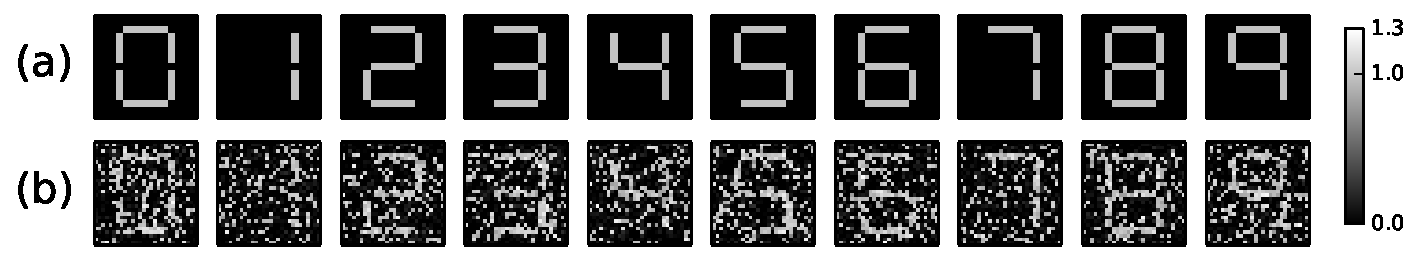
\includegraphics[width=0.8\columnwidth]{./fig/digit_data.pdf}
 \caption{
 (a) Templates. (b) Noisy samples. Each figure is of $28 \times 28$ pixels.
 }
 \label{fig:digit_data}
\end{figure}
% END OF FIGURE
%
% END OF PARAGRAPH

Using the artificial dataset above and the standard MNIST, we trained a feed-forward neural
network for the classification of ten numerics.
%
In Table~\ref{tab:NN_specification}, we provide the structure of the neural network and its performance over
each dataset.
%
For either dataset, the training was conducted via MSGD with constant
learning rate $\eta$.
%
%
We also adopted a dropout method~\cite{Hinton2012} only for the training
on the MNIST dataset.
%
The output from each unit in the final layer is given by the posterior
probability of each class $c$.
%
For computational purpose, we transform this output by $\log$:
%
\begin{align}
 f_{c}(\bvec{x}) := \log P(Y = c \,|\, \bvec{x}),
\end{align}
%
We then constructed the PSMs and the standard sensitivity map for the $f_c$
given above.
% Table 1
\begin{table}[htbp]
 \caption{Summary of training setups based on neural networks}
 \centering
 \begin{tabular}{lccccc}
  \hline
  \textbf{Data set} & \textbf{Architecture} & \textbf{Unit type} & \textbf{Dropout}
  & \textbf{Learning rate} & \textbf{Error[\%]} \\
  \hline
  Digital data & 784-500-10 & Logistic & No & 0.1 & 0.36  \\
  MNIST & 784-500-500-10 & ReLU & Yes &  0.1 & 1.37 \\
  \hline
 \end{tabular}
 \label{tab:NN_specification}
\end{table}
% END OF SUBSECTION

\subsection{PSA of the classifier trained on artificial dataset}
\label{sec:psa_art}
%
We will describe three ways in which the PSA can be superior to the
analysis based on standard sensitivity map.
% END OF PARAGRAPH

%%%  Result1: Positive negative %%%
Fig.\,\ref{fig:first_psm} compares the PSMs and standard
sensitivity maps, which were both
obtained from the common neural networks trained for the same
10-class classification problem.
%
The color intensity of $i$-th pixel represents the magnitude of $s_i$ or $v_i$.
%
Both maps capture the characters that the ``colorless''
rims and likewise ``colorless'' regions enclosed by edges are insignificant in the classification.
%
Note that the (first) PSM distinguishes the types of sensitivities by
their sign.
%
For each numeral, the PSM assigns opposite signs to ``the edges whose \textit{presence} is
crucial in the characterization of the very numeral'' and ``the edges
whose \textit{absence} is crucial in the numeral's characterization.''
%
This information is not featured in the standard sensitivity map.
%
For instance, in the sensitivity map for the numeral $1$, the two edges on the
right and the rest of the edges have the opposite sensitivity.
As a result, we can verify the red figure of $1$ in its PSM.
%
We are able to clearly identify the unbroken figures of $2,4,5$ and $9$ in their
corresponding PSM as well.
%
We see that, with the extra information
regarding the sign of the sensitivity over each pixel, PSM can provide
us with much richer information than the standard counterpart.
% Fig.1
\begin{figure}[htbp]
 \centering
 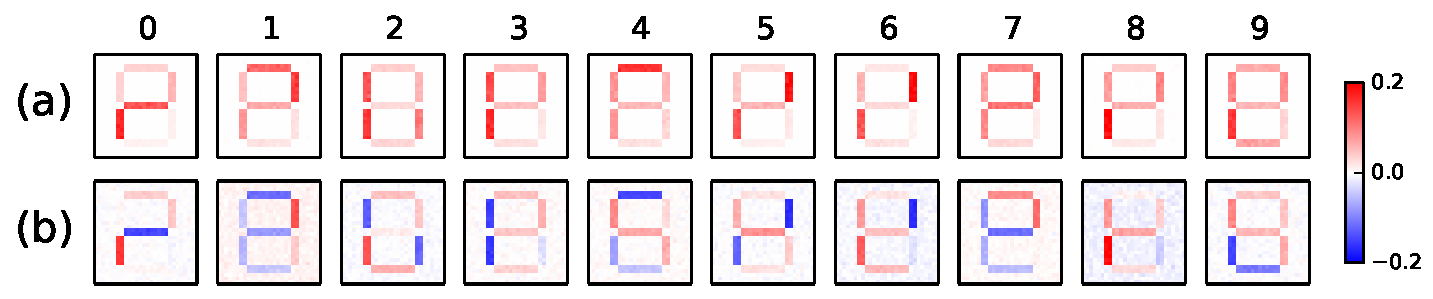
\includegraphics[width=0.9\columnwidth]{./fig/first_psm.pdf}
 \caption{(a) Standard sensitivity maps. (b) PSMs.
 }
 \label{fig:first_psm}
\end{figure}
% END OF PARAGRAPH

%%% RESULTS2: PSA %%%
Next, we will show the benefits of sub-principal sensitivity maps
computed from PSA.
%
Fig.\,3(a) shows the first PSM through the third PSM for the numerals $0$ and
$9$.\footnote{We list the PSMs for all the numerals ($0, \dots, 9$) in
the Appendix~\ref{sec:appendix_digit}.}
%
In order to show how this extra information benefits us in visualization
of the classification problem, we consider the following
``local'' sensitivity map integrated over the samples from a particular
pair of classes:
%
\begin{align}
\begin{split}
s_{c,c'}(\bvec{v}) := E_{q_{c, c'}} \left[ \left( \frac{\partial f_c (\bvec{x})}{\partial {\bvec{v}}} \right)^2 \right],
\end{split}  \label{def:l_psm}
\end{align}
%
where $q_{c, c'}$ is the empirical distribution over the set of samples
generated from the classes $c$ and $c'$.
%
To get the intuition about this value, note that the value for $(c, c') =
(9, 4)$ can also be pictorially written as
%
\begin{flalign}
  \lim_{\varepsilon \rightarrow 0}
 E_{\{9, 4\}} \left[
 \left(
  \frac
  {\log P \left(Y = \parbox{\bwcnine}{\usebox{\cnine}} |
  \parbox{\bwcnine}{\usebox{\sfour}} + \varepsilon \bvec{v} \right)
  - \log P \left(Y = \parbox{\bwcnine}{\usebox{\cnine}} |
  \parbox{\bwcnine}{\usebox{\sfour}} \right)}
  {\varepsilon}
  \right)^2
  \right],
\end{flalign}
%
where $\bvec{v}$ can be the third PSM of class 9, \parbox{\bwpninethird}{\usebox{\pninethird}}, for
example.
%
If $\bvec{v}_{k}$ is the $k$-th PSM of the classifier,
then $s_{c,c'}(\bvec{v}_{k})$ quantifies \textit{the sensitivity of the machine's
answer to the binary classification problem of ``$c$ vs $c'$''} with
respect to the perturbation of the input in the direction of $\bvec{v}_{k}$.
%
By looking at this value for each $k$, we may visualize the ways that the classifier
deals with the binary classification problem.  Such visualization may aid us
in learning from the classifiers the way to distinguish one class from another.
%
Fig.\,3(b) shows the
values of $s_{c,c'}(\bvec{v}_{k})$ for $c \in \{0, 9\}$ and $k \in \{1,\dots,10 \}$.
%
We could see in the figure that, for the case of
$(c, c') = (9, 4)$, $s_{c,c'}(\bvec{v}_{3})$ was larger than
$s_{c,c'}(\bvec{v}_{1})$.
%
This suggests that the third PSM is more helpful than the first PSM for
distinguishing $4$ from $9$.
%
We can actually verify this fact by observing that the third PSM is
especially intense at the top most edge, which can alone differentiate $4$ from $9$.
%
We are able to confirm many other cases in which the sub-principal sensitivity maps were
more helpful in capturing the characters in binary classification problems than the first PSM.
%
Thus, PSA can provide us with the knowledge of the classifiers
that was inaccessible with the previous method based on the standard
sensitivity map.
% Figure 3
\begin{figure}[htbp]
\centering
 \begin{minipage}[t]{0.35\columnwidth}
  \centering
   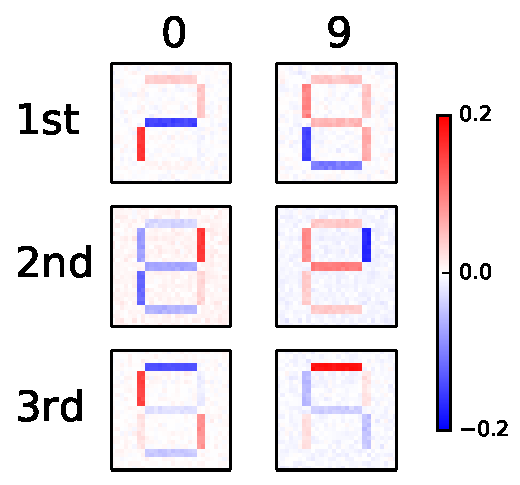
\includegraphics[clip, width=1.\columnwidth]{./fig/fig3a.pdf}
  \hspace{1.6cm} \textsf{(a)}
  \end{minipage}
 \begin{minipage}[t]{0.6\columnwidth}
  \centering
   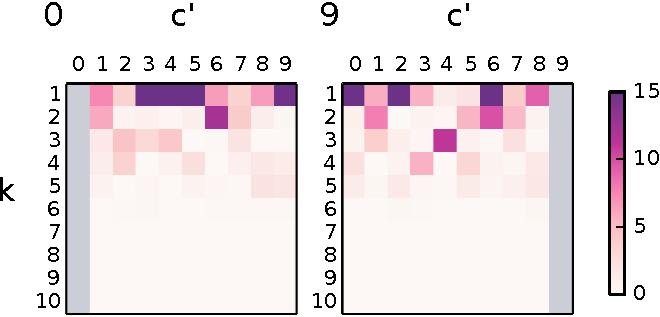
\includegraphics[clip, width=1.\columnwidth]{./fig/fig3b_modified.pdf}
  \hspace{1.6cm} \textsf{(b)}
 \end{minipage}
  \label{fig:digit09}
 \caption{(a) First, second and third PSMs of the classifier outputs $f_c$ for the numerals
 $0$ and $9$. (b) $s_{c, c'}(\bvec{v}_{k})$ for $c \in \{0, 9\}$, $k \in
 \{1, \dots, 10\}$, and $c' \in \{0, \dots, 9\} \backslash \{c\}$.}
\end{figure}
% END

%%%%%%%%%%%%%%%%%%%%%%%%%%%%%%%%%%%%%%%%%%%%%%%%%%%%%%%%%%%%%%%%%%%%%%%%%%%%%%%%%%%%%%%%%
% RESULTS3: Sparse PSA
%%%%%%%%%%%%%%%%%%%%%%%%%%%%%%%%%%%%%%%%%%%%%%%%%%%%%%%%%%%%%%%%%%%%%%%%%%%%%%%%%%%%%%%%%
Finally, we demonstrate the usefulness of formulation~\eqref{eq:PSA} in
the construction of sparse and intuitive sensitivity map.
%
Fig.\,\ref{fig:spsm_digit} depicts the sensitivity maps obtained from the
application of our sparse PSA in~\eqref{eq:sparsePSA} to the data above.
%
Note that the sparse PSA not only washes away rather irrelevant
pixels from the canvas, but it also assigns very high intensity to essential pixels.
%
With these ``localized'' maps, we can better understand the discriminative features
utilized by the trained classifiers.
% Figure 4
\begin{figure}[htbp]
 \centering
 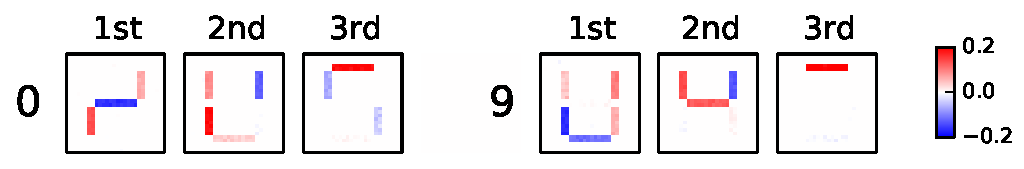
\includegraphics[width=0.8\columnwidth]{./fig/fig4.pdf}
 \caption{
 Results of the sparse PSA on the classifiers $f_c$ with $r =
 3$ for the numerals $0$ and $9$.
 We ranked the $3$ basis elements in the increasing order of $s(\bvec{v})$.
 We selected the regularization term of  $\lambda = 5$,
 and each PSM was normalized so that its $L_2$ norm was $1$.
 }
 \label{fig:spsm_digit}
\end{figure}
% END OF SUBSECTION

%%%%%%%%%%%%%%%%%%%%%%%%%%%%%%%%%%%%%%%%%%%%%%%%%%%%%%%%%%%%%%%%%%%%%%%%%%%%%%%%%%%%%%%%%
\subsection{PSA of the classifier trained on MNIST dataset}
%%%%%%%%%%%%%%%%%%%%%%%%%%%%%%%%%%%%%%%%%%%%%%%%%%%%%%%%%%%%%%%%%%%%%%%%%%%%%%%%%%%%%%%%%
We trained a nonlinear neural network-based classifier on the MNIST
dataset, which consists of hand-written digits from $0$ through $9$.
%
We then analyzed the trained classifier with our PSA.
%
This dataset illuminates a particular challenge to be confronted in the application of the PSA.
%
By default, hand-written objects do not share common displacement and orientation.
%
Without an appropriate registration of input space,
the meaning of each pixel can vary across the samples, making the
visualization unintuitive.
%
This is typical in some of the real-world classification problems.
%
In the fields of applied science, standard registration procedure is
often applied to the dataset before the construction of the classifiers.
%
For example, in neuroimaging, one partitions the image data into anatomical
regions after registration based on the standard brain,
and represents each one of them by a group of voxels.
%
In other areas of science, one does not necessarily have to face such problems.
%
In genetics, data can be naturally partitioned into genes~\cite{Yukinawa2009}.
%
Likewise, in meteorology, 3D dataset is often translated into voxel
structures, and a group of voxels may represent geographical region of
specific terrain~\cite{Kontos2005}.
%
In this light, the digit recognition in unregistered MNIST data may not
be an appropriate example for showing the effectiveness of our visualization method.
For the reason that we will explain later, registration of multiclass
dataset like MNIST can be difficult.
%
We chose MNIST dataset here because it is familiar in the community of
machine learning.
% END OF PARAGRAPH

% Fig
Fig.\,\ref{fig:psms_mnist} summarizes the results.
%
Both the standard sensitivity map and the PSM were able to
capture the character that outer rims are rather useless in the classification.
% Figure 5
\begin{figure}[htb]
 \centering
 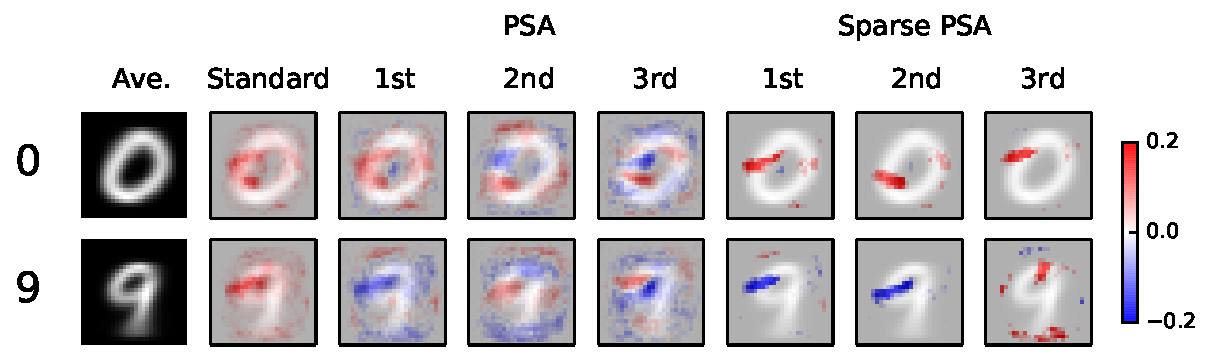
\includegraphics[width=0.8\columnwidth]{./fig/fig5a.pdf}
 \caption{Standard sensitivity maps, PSMs, and sparse PSMs for
 $c \in \{0, 9\}$, $k \in \{1, 2, 3\}$, and $c' \in \{0, \dots
 ,9\} \backslash \{c\}$.
 Ave. stands for the average of the testing dataset for the corresponding numerals.}
 \label{fig:psms_mnist}
\end{figure}
% END OF PARAGRAPH

% local
Fig.\,\ref{fig:local_s_mnist} shows the values of $s_{c,c'}(\bvec{v}_{k})$.
We can verify that small numbers of PSMs are complementing each other
in their contributions to the binary classifications.
% Figure 6
\begin{figure}[htb]
 \centering
 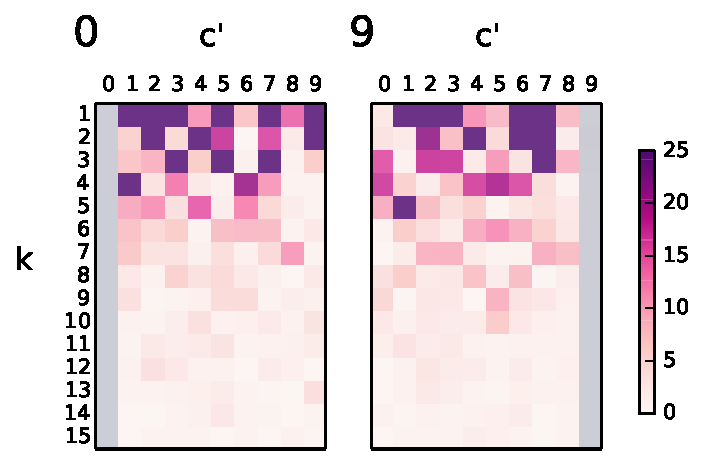
\includegraphics[width=7cm]{./fig/fig5b.pdf}
 \caption{$s_{c, c'}(\bvec{v}_{k})$ for $c \in \{0, 9\}$, $k \in
 \{1, \dots, 15\}$, and $c' \in \{0, \dots, 9\} \backslash \{c\}$.}
 \label{fig:local_s_mnist}
\end{figure}
% END OF PARAGRAPH

%%% Sparse PSMA on MNIST %%%
We also applied sparse PSA to the classifier with $r = 3$ and $\lambda =
40$ (see Fig.\,\ref{fig:psms_mnist}).
We see that the sparse PSA highlights the essential pixels much more clearly
than the normal PSA.
% END OF PARAGRAPH

%%% Excuse %%%
Since the orientation and position of each numeral pattern
varies across the samples in this dataset,
input dimensions hold different meanings in different samples.
%
To perform more effective visualization,
we would need registration to adjust each numeral pattern
to a common standard template.
%
This problem might not be straightforward, since one must prepare
different templates for different numeral patterns.
An elegant standardization suitable for our PSA-based visualization
remains as a future study.
% END OF SECTION
